\documentclass[11pt]{article}
\addtolength{\oddsidemargin}{-1.cm}
\addtolength{\textwidth}{2cm}
\addtolength{\topmargin}{-2cm}
\addtolength{\textheight}{3.5cm}

\usepackage[pdftex]{graphicx}
\usepackage{hyperref}
\usepackage{cite}
\hypersetup{
	colorlinks=true,
	linkcolor=black,
	filecolor=magenta,
	urlcolor=cyan,
}

% define the title
\author{Team Bravo}
\title{Software Requirements Specification and Technology Neutral Process Design and Software Architecture Documentation}
\begin{document}
	\setlength{\parskip}{6pt}
	
	% generates the title
	\begin{titlepage}
	
	\begin{center}
		% Upper part of the page       
		
\includegraphics[width=1\textwidth]{../Diagrams/Images/University_of_Pretoria_Logo.PNG}\\[0.5cm]    
		\textsc{\LARGE Department of Computer Science}\\[0.5cm]
		\textsc{\Large COS 301}\\[0.5cm]
		\textsc{\Large Mini Project} \nocite{ref}\\[0.5cm]
		% Title
		\rule{\linewidth}{0.5mm} \\[0.4cm]
		{ \huge \bfseries Software Requirements Specification and Technology Neutral Process Design and Software Architecture Documentation}\\[0.2cm]
		\rule{\linewidth}{0.5mm} \\[1cm]
		
		% Author and supervisor
		\textsc{\Large Team Bravo}\\[1cm]
		
		
		\begin{minipage}{0.4\textwidth}
			\begin{flushleft} \large
				\emph{Student:}\\[0.75cm]
				Daniel {King}
			\end{flushleft}
		\end{minipage}
		\begin{minipage}{0.4\textwidth}
			\begin{flushright} \large
				\emph{Student number:} \\[0.75cm]
				u13307607
			\end{flushright}
		\end{minipage}
		
		
		\begin{minipage}{0.4\textwidth}
			\begin{flushleft} \large
				\emph{} \\
				Azhar {Mohungoo }
			\end{flushleft}
		\end{minipage}
		\begin{minipage}{0.4\textwidth}
			\begin{flushright} \large
				\emph{} \\
				u12239799
			\end{flushright}
		\end{minipage}
		
		
		\begin{minipage}{0.4\textwidth}
			\begin{flushleft} \large
				Andreas {du Preez}
			\end{flushleft}
		\end{minipage}
		\begin{minipage}{0.4\textwidth}
			\begin{flushright} \large
				\emph{} \\
				u12207871 
			\end{flushright}
		\end{minipage}
		
		
		\begin{minipage}{0.4\textwidth}
			\begin{flushleft} \large
				Banele {Nxumalo}
			\end{flushleft}
		\end{minipage}
		\begin{minipage}{0.4\textwidth}
			\begin{flushright} \large
				\emph{} \\
				u12201911 
			\end{flushright}
		\end{minipage}
		
		
		\begin{minipage}{0.4\textwidth}
			\begin{flushleft} \large
				Frederic {Ehlers}
			\end{flushleft}
		\end{minipage}
		\begin{minipage}{0.4\textwidth}
			\begin{flushright} \large
				\emph{} \\
				u11061112  
			\end{flushright}
		\end{minipage}
		
		
		\begin{minipage}{0.4\textwidth}
			\begin{flushleft} \large
				Diana {Obo}
			\end{flushleft}
		\end{minipage}
		\begin{minipage}{0.4\textwidth}
			\begin{flushright} \large
				\emph{} \\
				u13134885
			\end{flushright}
		\end{minipage}
		
		
		\begin{minipage}{0.4\textwidth}
			\begin{flushleft} \large
				Bilal {Muhammad}
			\end{flushleft}
		\end{minipage}
		\begin{minipage}{0.4\textwidth}
			\begin{flushright} \large
				\emph{} \\
				u13080335
			\end{flushright}
		\end{minipage}
		\vfill
		
	\end{center}
\end{titlepage}
	
	\renewcommand{\thesection}{\arabic{section}}
	\newpage
	
	\tableofcontents
	
	\section{Introduction}
	
	This document aims to specify the functional and non-functional requirements of a document archiving system, as specified by Ms Vreda Pieterse of the Computer Science Department.
	
	It will serve as a means of communication between the client and developers as well as providing an elaboration and a clear discription of it's implementation specifications.
	
	\section{Vision}
	
	We intend to create a system that will allow authors and their co-authors to work on their research papers in an environment that reassures collaborative work, which in turn diminishes the time spent on papers with multiple authors. The following are what we plan to achieve:
	
	\begin{itemize}
		\item Keep track of research papers.
		\item View meta-data of research papers.
		\item Allow multiple authors to collaborate on the same research paper.
		\item Different levels of authority, i.e. Admin, (Co)Author, User.
		\item View and edit the details, of a text based profile, of different researchers.
		\item Implemention as a website and an android application.
	\end{itemize}
	
	\section{Background}
	
	We live in a world where time is valuable. We would like to do as much as we possibly can in the shortest amount of time. And if that's not possible, we work in teams to ensure that we achieve that goal.
	
	Reseacher papers tend to be fairly lengthy, and if completed by only one author, it could be quite a tedious process. Hence we propose a system which would make the storage and collaboration of research articles and papers effortless by producing an archive system.

	\newpage
	
	\section{Architecture requirements}
	
	\subsection{Architecture requirements}
		\subsection{Access channel requirements}
			The different access channels for the system will be as follows:
		\subsubsection{Web Application}
			The system can be used via a web application that uses RESTful web services and bootstrap technology. The system will be fully supported on the following web browsers:
				\begin{itemize}
					\item Chrome 7.0.517 and up
					\item Firefox 3.6 and up
					\item Safari 4 and up
					\item Edge
				\end{itemize}
			Bootstrap will be used so that the web application will also be accessible by mobile web browsers that support HTML5 and JavaScript technology.
		\subsubsection{Mobile Application}
			The system will also be accessible via a mobile application and will be operational on the following mobile operating systems:
				\begin{itemize}
					\item Android 4.0 (Ice Cream Sandwich) and up.
				\end{itemize}
	
	\subsubsection{Architectural scope}
		\begin{itemize}
			\item stuffs
		\end{itemize}
	
	\subsection{Quality requirements}
		\begin{itemize}
			\item Security - The system shall identify all of its client applications before allowing them access to those enities. Possible measurement methods: Success rate in authentication, percentage of successful attacks, encryption level and probability/time/resources needed to attack the system.
			\item Usability - The degree of ease of use and training needed for end users. Possible measurement methods: Time it took a user to find a report (search functionality), percentage of deadlines met (notification functionality) and time it took a user to perform certain tasks.
			\item Auditability - The degree to which transactions can be traced. Possible measurement methods: The number and precision of logs generated in a period of time (metadata accessed/deleted/added).
			\item Portability - Measure ability of the system to run under different computing environments. Possible measurement methods: Number of targeted software environments (ie different browsers and operating systems) and proportion of platform specific functionality.
			\item Maintainability - Measures ability to make changes quickly and cost effectively. Possible measurement methods: Degree of complexity to make changes to the format of the metadata and mean time to add or change certain functionalities (ie new report types and new types of users).
			\item Availability - Percentage of time that the system is up and running correctly. Possible measurement methods: Length of time between failures and length of time needed to resume operation after a failure.
			\item Performance - Possible measurement methods: How well the system perform under high workload and number of events processed/denied in some interval of time.
		\end{itemize}
	
	\subsection{Integration and access channel requirements}
		\subsubsection{Integration channels}
			\begin{itemize}
				\item System will be integrated on two platforms: a website and an android application.
			\end{itemize}
		\subsubsection{Protocols}
			\begin{itemize}
				\item Protocols needed for the website: HTTPS, Data Query Protocol
				\item Protocols needed for the application: Session Initiation Protocol (SIP)
			\end{itemize}
		\subsubsection{Integration quality requirements}
			\begin{itemize}
				\item Reliability - The service must not crash, it must run effectively and efficiently allowing users to make use of the service at all times.
				\item Auditability - Have logs record all activity that occurs thus all actions and occurrences can be traced.
				\item Security - Giving the users reassurance that the system will protect their details and content. Allow secure and safe communication between user and the system.
				\item Maintainability - Provide easy, effective and efficient maintenance to the system allowing minimal or no downtime of the system.
				\item Usability - Allow users to use the system with ease and minimal need for tutorials. Ensure that the system is self-explanatory, efficient and effective.
				\item Portability - To provide compatibility with as many systems as possible without integration failure or function failure.
				\item Availability - Minimise downtime of the system. Quick recoveries from crashes, preventive measures to minimise chances of system crash.
				\item Performance - The rate of work done when the system has either a high or low workload and minimise amount of denied events.
				\item Seamless transitions between platforms - Implementation between the integrated platforms must not vary greatly to avoid confusion and allow ease of use.
			\end{itemize}

	\subsection{Architecture constraints}
		\begin{itemize}
			\item The platform must exist in 2 mediums, namely web and android application.
			\item It is an internal network to be used by the Computer Science department, so it need not to source any information from the web.
			\item Any form of database can be used, but the team has decided that MySQL would be the best option from the current skillset.
			\item PHP and JavaScript will be used for the web and Android Studio for the android application.
			\item The system should cater for and including 100 users as a maximum.
			\item There should be a log that records all activity on the system
		\end{itemize}

	
	\subsection{Architectural patterns or styles}
	\subsubsection{MVC architecture}
	The MVC (Model View Control) architecture allows change to the system's state. The model is completed through a common interface(the control). The view is where developments are made to user interfaces and these changes are independent to the system providing extensibility at a low cost.
	
	Reasons to use MVC:	
	\begin{itemize}
		\item It encapsulates the interaction from the user and transforms those interactions, in the form of requests into business logic that interacts with the system mode to produce reponses. 
		\item A multi-layered approach encapsulated by the MVC which enables the separation of business logic providing the need for sub-systems and internal and external APIs.  

	\end{itemize}
	The MVC architecture  will be based on SOA (Service Oriented Architecture) reference architecture. It is a loosely-coupled architecture where services exist independently from each other. They communicate with each other by means of protocols and standard-based interfaces such as SOAP and XML schema to define messages passed between objects. Services and functionality can easily be added to the existing system during progession. 

	Reasons to use SOA:
	\begin{itemize}
		\item Reuse of objects
		\item Flexible and agile
		\item Simplicity of implementation
		\item System is open to change and easy alteration

	\end{itemize}
	
	\subsubsection{Three-tier architecture}
	The three-tier architecture is a client-server software architecture pattern where the user interface (presentation), functional process logic(business rules), computer data storage and data access are developed and maintained as independent modules, most often on separate platforms.

	\subsection{Architectural tactics or strategies}
	
		Availability is best defined by the proportion of time a system is functional and working as required. It can be affected by system errors, infrastructure problems, malicious attacks and system load. Here are some key issues:
		\begin{itemize}
			\item The server on which the database is kept can fail or become unresponsive, causing the entire system to fail. We will have to consider how to design failover support in the system. For example, we can use Network Load Balancing for Web servers to distribute the load and prevent requests being directed to a server that is down. Also, consider using a RAID mechanism to mitigate system failure in the event of a disk failure.
			
			\item Denial of service attacks, which prevent authorised users from accessing the system, can interrupt operations if the system cannot handle massive loads in a correct and timely manner, often due to the processing time required, or network configuration and congestion. To minimize interruption from such attacks, identify malicious behaviour, use application instrumentation to expose unintended behaviour, and implement comprehensive data validation. We will consider using the Circuit Breaker or Bulkhead patterns to increase system resiliency.
		\end{itemize}
		
		Conceptual integrity is the consistency and coherence of the overall design. This means that we have to be consistent in our various modules’ designs as well as coding styles and variable names. A coherent system is one that is easy to maintain because you will know what is consistent in the modules. Things to look at:
		\begin{itemize}
			\item Lack of collaboration and communication between different groups involved in the application lifecycle. We should establish a development process integrated with tools to facilitate process workflow, communication, and collaboration.
			
			\item Lack of design and coding standards. A guideline for design and coding standards should be made, and we can incorporate code reviews into our development process to ensure guidelines are followed.
		\end{itemize}
		
		Maintainability is the ability of the system to undergo changes with a degree of ease. These changes could impact components, services, features, and interfaces when adding or changing the application’s functionality in order to fix errors, or to meet new business requirements. We will tackle this challenge in the following way:
		\begin{itemize}
			\item This documentation will serve as the basic requirements of the system which will make it easier to upgrade and maintain the system at all times.
			
			\item The technologies we will be using like PHP, JavaScript, etc are well known languages in the programming world, making it easy to find programmers that can interpret existing code as well as add on to it.
			
			\item Logical errors can be difficult to trace in such huge systems, and can cause unnecessary dependencies on other components. Rather we will try to design components so that they are cohesive by having low coupling and thus reducing dependencies.
		\end{itemize}
		
			Manageability is about how easy it is for the system administrators (tech team) to manage the application. This is important for key factors like monitoring systems, debugging and performance tuning. We will try to tackle this with the following approach:
			\begin{itemize}
				\item System logs should be backed up yearly, making sure that they are safely kept on a machine other than the server.
				
				\item We should capture and report sufficient information about errors and state changes in order to enable accurate monitoring, debugging, and management. Also, we should consider creating management packs that administrators can use in their monitoring environments to manage the application.
				
				\item We should be able to create snapshots of the system so that in case of system failure we can revert to the most recent system state instead of having lost all previous work.
			\end{itemize}

	\subsection{Use of reference architectures and frameworks}
	
	\subsection{Access and integration channels}
	
	\begin{itemize}
		\item API's?
		\item Simple Access Project Protocol (SOAP) is a protocol which allows programs that run on different operating system to communicate using HTTP and XML. It's platform and language independent. It's quite useful in handling asynchronous processing and supports many other protocols and technologies
		\item The system will be accessible by using a web interface which is bootstraped to cater for all devices of different sizes
		\item Access to the system will be provided using the HTTPS protocol to ensure security, along with IPsec (Internet Protocol Security) which will allow for a secure IP and to ensure that no malicious data is sent to the servers
		\item WSDL (Web Service Definition Language)
		\item IDL (Interactive Data Language)
		\item PHP backend
		\item MySQL database
		\item RESTful web services
	\end{itemize}
	
	\newpage
	
	\section{Functional requirements and application design}
	
	\subsection{Use case prioritization}
	This section specifies the level of importance of different use cases, prioritized in terms of the following 3 catogories: Critical, Important and Nice-To-Have. Each of which has a lesser importance than the previous one.
	
	\subsubsection{Critical:}
	\begin{itemize}
		\item User gateaway
		\begin{itemize}
			\item Register user
			\item Login user
		\end{itemize}
		\item Research paper management
		\begin{itemize}
			\item View paper
			\item Publish paper
			\item Terminate paper
			\item Assign research paper's conference venue
			\item View research paper's venue
		\end{itemize}
		\item User account management
		\begin{itemize}
			\item View user account
			\item Remove account
			\item Create new account
			\item Search user
			\item Modify account
			\item Assign co-author
		\end{itemize}
		\item Log services
		\begin{itemize}
			\item View recent activities
			\item System events
			\item Determine date and time
			\item Identify user
		\end{itemize}
		\item Other
		\begin{itemize}
			\item System should only allow one primary author for each research paper. The rest should be co-authors
			\item Superuser, one to be above all other users to have complete control and access to the entire system
			\item Only metedata of the document will be posted, no documents will be posted
			\item Research documents are archived rather than deleted
		\end{itemize}
		
	\end{itemize}
	
	\subsubsection{Important:}
	\begin{itemize}
		\item Notification Services
		\begin{itemize}
			\item Create notification
		\end{itemize}
		\item Archival Services
		\begin{itemize}
			\item Terminate paper
			\item Revive paper
		\end{itemize}
	\end{itemize}
	\begin{itemize}
		\item Units accumulated from work on papers is reflected on the user's profile
	\end{itemize}
	
	\subsubsection{Nice-To-Have:}
	\begin{itemize}
		\item Users can search for other users attending the same conference
		\item Data representation via bar charts of the units accumulated by researchers throughout the past years
	\end{itemize}
	
	\newpage
	
	\subsection{Use case/Services contracts}
		\subsubsection{Login user}
		\begin{itemize}
			\item \textbf{Description: }The ability for a user to login to the system
			\item \textbf{Pre-Condition: }A user name and password must be provided by the user attempting to login. The username must exist in the database and the password needs to be the same as the one found within the database. 
			\item \textbf{Post-Condition: }The user will be notified the login was successful and now has the privledges associated with the account.
		\end{itemize}
		\begin{center}
			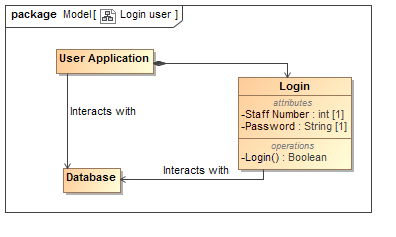
\includegraphics[width=\textwidth]{../Diagrams/DomainModel/Loginuser.png}\\[0.5cm]
		\end{center}
		\newpage
		 \subsubsection{Register User}
		\begin{itemize}
			\item \textbf{Description: }The ability to create a new account within the system
			\item \textbf{Pre-Condition: }The user must provide a username, password and email address that will be associated with the created account. The username must also not already exist within the database. 
			\item \textbf{Post-Condition: }The account needs to be created and exist within the database
		\end{itemize}
		\begin{center}
			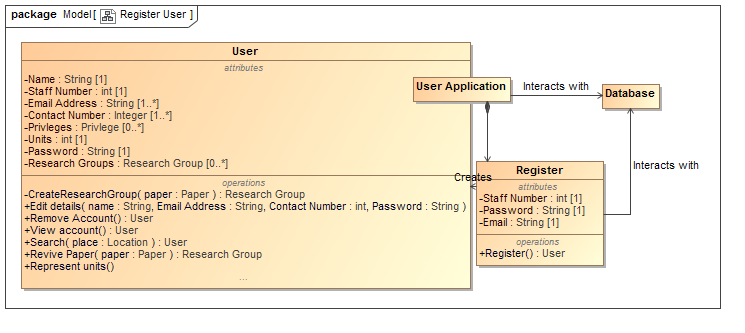
\includegraphics[width=\textwidth]{../Diagrams/DomainModel/RegisterUser.png}\\[0.5cm]
		\end{center}
		\newpage
		\subsubsection{View paper}
		\begin{itemize}
			\item \textbf{Description: }The ability to view the meta-data related to a research paper
			\item \textbf{Pre-Condition: }The user attempting to view the paper must be an author of the paper or have sufficent privledge.
			\item \textbf{Post-Condition: }The data of the paper in question must be displayed to the user.
		\end{itemize}
		\begin{center}
			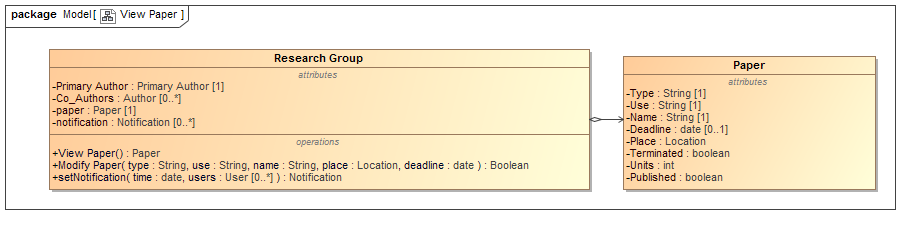
\includegraphics[width=\textwidth]{../Diagrams/DomainModel/ViewPaper.png}\\[0.5cm]
		\end{center}
		\newpage
		\subsubsection{Modify paper}
		\begin{itemize}
			\item \textbf{Description: }The ability to edit the meta-data related to a research paper.
			\item \textbf{Pre-Condition: }The user attempting to edit the paper must be an author of the paper or have sufficent privledge.
			\item \textbf{Post-Condition: }The paper's meta-data needs to be altered in the desired way.
		\end{itemize}
		\begin{center}
			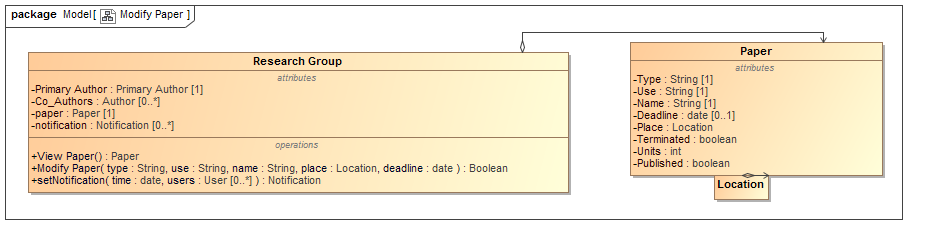
\includegraphics[width=\textwidth]{../Diagrams/DomainModel/ModifyPaper.png}\\[0.5cm]
		\end{center}
		\newpage
		\subsubsection{Publish paper}
		\begin{itemize}
			\item \textbf{Description: }The ability to set a paper within the system as published and discontinue work on it.
			\item \textbf{Pre-Condition: }A user with sufficient priveledge should be making this action
			\item \textbf{Post-Condition: }The paper is set as published and the group is dissolved.
		\end{itemize}
		\begin{center}
			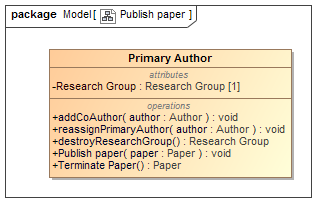
\includegraphics[width=\textwidth]{../Diagrams/DomainModel/Publishpaper.png}\\[0.5cm]
		\end{center}
		\newpage
		\subsubsection{Terminate paper}
		\begin{itemize}
			\item \textbf{Description: }The paper is discontinued by the current research group
			\item \textbf{Pre-Condition: }The request has to be made by the primary-author, the admin, the Superuser or the Head of Department
			\item \textbf{Post-Condition: }The paper is listed as discontinued
		\end{itemize}
		\begin{center}
			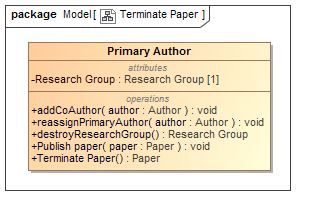
\includegraphics[width=\textwidth]{../Diagrams/DomainModel/TerminatePaper.png}\\[0.5cm]
		\end{center}
		\newpage
		\subsubsection{Edit Account}
		\begin{itemize}
			\item \textbf{Description: }The ability for users to edit their profiles
			\item \textbf{Pre-Condition: }The user attempting to edit the profile must either have sufficient priveledge or must be the owner of the account
			\item \textbf{Post-Condition: }The profile has been edited in the desired way
		\end{itemize}
		\begin{center}
			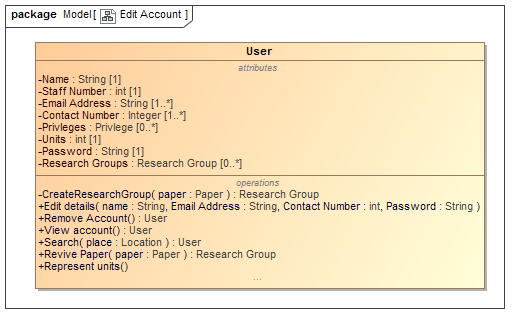
\includegraphics[width=\textwidth]{../Diagrams/DomainModel/EditAccount.png}\\[0.5cm]
		\end{center}
		\newpage
		\subsubsection{Remove account}
		\begin{itemize}
			\item \textbf{Description: }Delete a user account from the system
			\item \textbf{Pre-Condition: }The user attempting to delete the profile must either have sufficient priveledge or must be the owner of the account
			\item \textbf{Post-Condition: }The profile no longer exists within the system
		\end{itemize}
		\begin{center}
			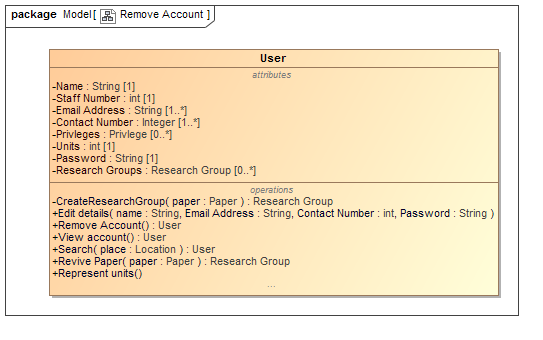
\includegraphics[width=\textwidth]{../Diagrams/DomainModel/RemoveAccount.png}\\[0.5cm]
		\end{center}
		\newpage
		\subsubsection{View user account}
		\begin{itemize}
			\item \textbf{Description: }The ability for a user to view an account
			\item \textbf{Pre-Condition: }The user must be logged into their account or the user attempting to view the account must be an admin, super admin, or head of department.
			\item \textbf{Post-Condition: }The user's account needs to be displayed for the requesting user
		\end{itemize}
		\begin{center}
			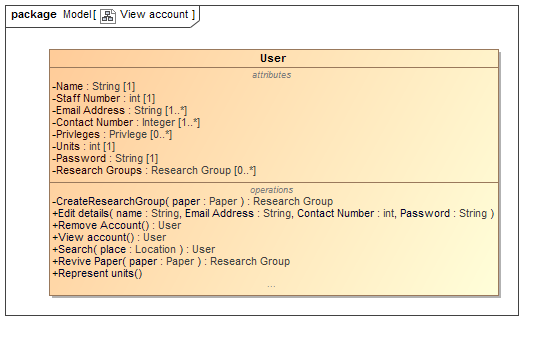
\includegraphics[width=\textwidth]{../Diagrams/DomainModel/Viewaccount.png}\\[0.5cm]
		\end{center}
		\newpage
		\subsubsection{Search user}
		\begin{itemize}
			\item \textbf{Description: }The ability to search for users working on paper's for the same conference as well as admins, Superusers and the Head of Department to search for users based on certain criteria
			\item \textbf{Pre-Condition: }The criteria for the desired group of users must be specified
			\item \textbf{Post-Condition: }The user/s are presented to the user requesting
		\end{itemize}
		\begin{center}
			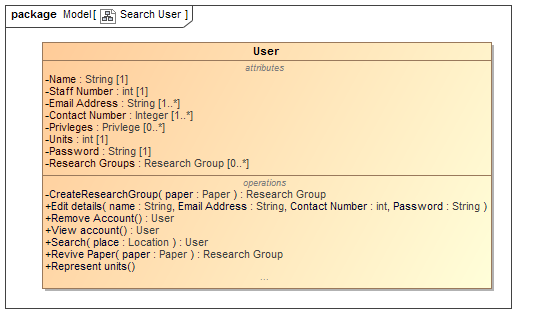
\includegraphics[width=\textwidth]{../Diagrams/DomainModel/SearchUser.png}\\[0.5cm]
		\end{center}
		\newpage
		\subsubsection{Assign co-author}
		\begin{itemize}
			\item \textbf{Description: }A co-author is assigned to a research group
			\item \textbf{Pre-Condition: }The user assigning the co-author must be a primary-author/admin/Superuser or Head of Department
			\item \textbf{Post-Condition: }The co-author is linked to the research group
		\end{itemize}
		\begin{center}
			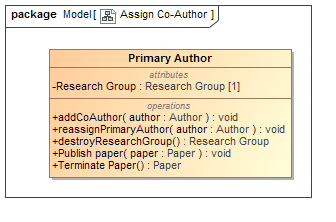
\includegraphics[width=\textwidth]{../Diagrams/DomainModel/AssignCoAuthor.png}\\[0.5cm]
		\end{center}
		\newpage
		\subsubsection{View recent activities}
		\begin{itemize}
			\item \textbf{Description: }The ability to view recent actions taken by the user on the system
			\item \textbf{Pre-Condition: }User requesting must be of sufficient priveledge
			\item \textbf{Post-Condition: }The activities are presented to the user requesting them
		\end{itemize}
		\begin{center}
			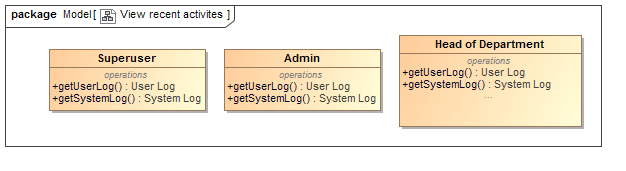
\includegraphics[width=\textwidth]{../Diagrams/DomainModel/Viewrecentactivites.png}\\[0.5cm]
		\end{center}
		\newpage
		\subsubsection{System events}
		\begin{itemize}
			\item \textbf{Description: }The ability to view logs of events that have taken place within the system
			\item \textbf{Pre-Condition: }User requesting must be an Admin, Superuser or Head of Department
			\item \textbf{Post-Condition: }The log of system events is presented to the user
		\end{itemize}
		\begin{center}
			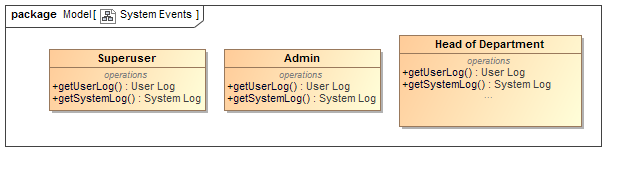
\includegraphics[width=\textwidth]{../Diagrams/DomainModel/SystemEvents.png}\\[0.5cm]
		\end{center}
		\newpage
		\subsubsection{Set notification}
		\begin{itemize}
			\item \textbf{Description: }The ability to set who receives a notification as well as when the notification should be issued
			\item \textbf{Pre-Condition: }The user setting the notification must be a Primary Author, Admin, Superuser or Head of Department
			\item \textbf{Post-Condition: }The notification is set and will email the specified user at the specified time/s.
		\end{itemize}
		\begin{center}
			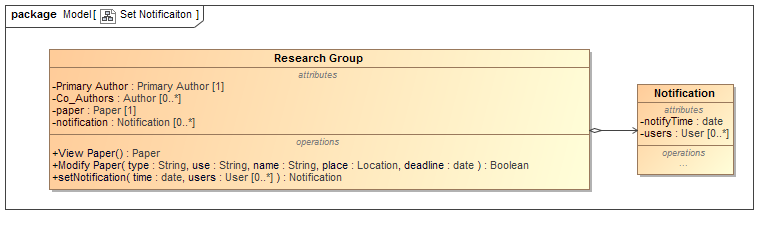
\includegraphics[width=\textwidth]{../Diagrams/DomainModel/SetNotificaiton.png}\\[0.5cm]
		\end{center}
		\newpage
		\subsubsection{Revive paper}
		\begin{itemize}
			\item \textbf{Description: }Assign a terminated paper to a new research group
			\item \textbf{Pre-Condition: }The terminated paper must exist within the system
			\item \textbf{Post-Condition: }A new research group is created with the requesting user as the primary-author
		\end{itemize}
		\begin{center}
			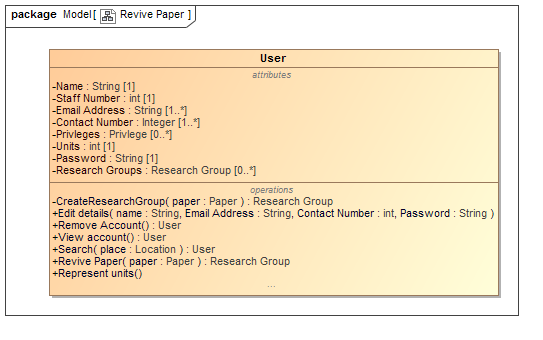
\includegraphics[width=\textwidth]{../Diagrams/DomainModel/RevivePaper.png}\\[0.5cm]
		\end{center}
		\newpage
		\subsubsection{Units accumulated from work on papers is reflected on ther user's profile}
		\begin{itemize}
			\item \textbf{Description: }Units accumulated from work on papers is reflected on ther user's profile
			\item \textbf{Pre-Condition: }A paper worth a certain number of units must be published and the user needs to be an author of the paper.
			\item \textbf{Post-Condition: }The units are added to the user's profile and displayed when the profile is viewed
		\end{itemize}
		\begin{center}
			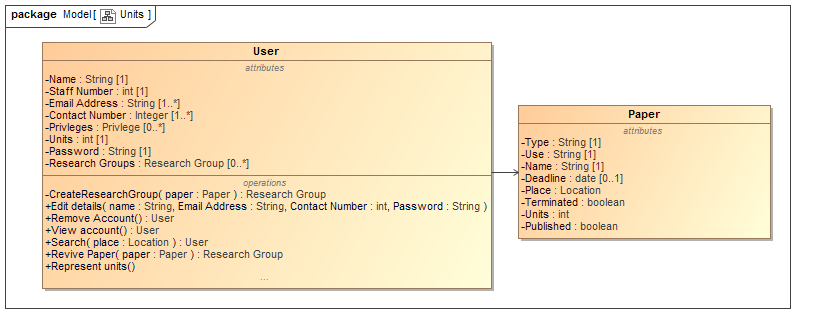
\includegraphics[width=\textwidth]{../Diagrams/DomainModel/Units.png}\\[0.5cm]
		\end{center}
		\newpage
		\subsubsection{Data representation of units accumulated}
		\begin{itemize}
			\item \textbf{Description: }A bar chart representation of the units a user has accumulated over time
			\item \textbf{Pre-Condition: }The user must exist and the user requesting to view the representation must be the owner of the account, an Admin, Superuser or HoD.
			\item \textbf{Post-Condition: }The bar chart is presented to the requesting user.
		\end{itemize}
		\begin{center}
			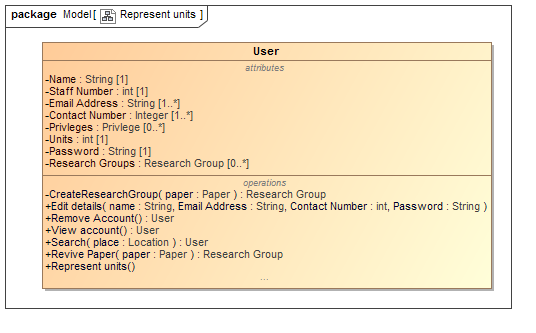
\includegraphics[width=\textwidth]{../Diagrams/DomainModel/Representunits.png}\\[0.5cm]
		\end{center}
	
	\subsection{Required functionality}
	
	
	\subsubsection{User Gateaway}
	\begin{center}
		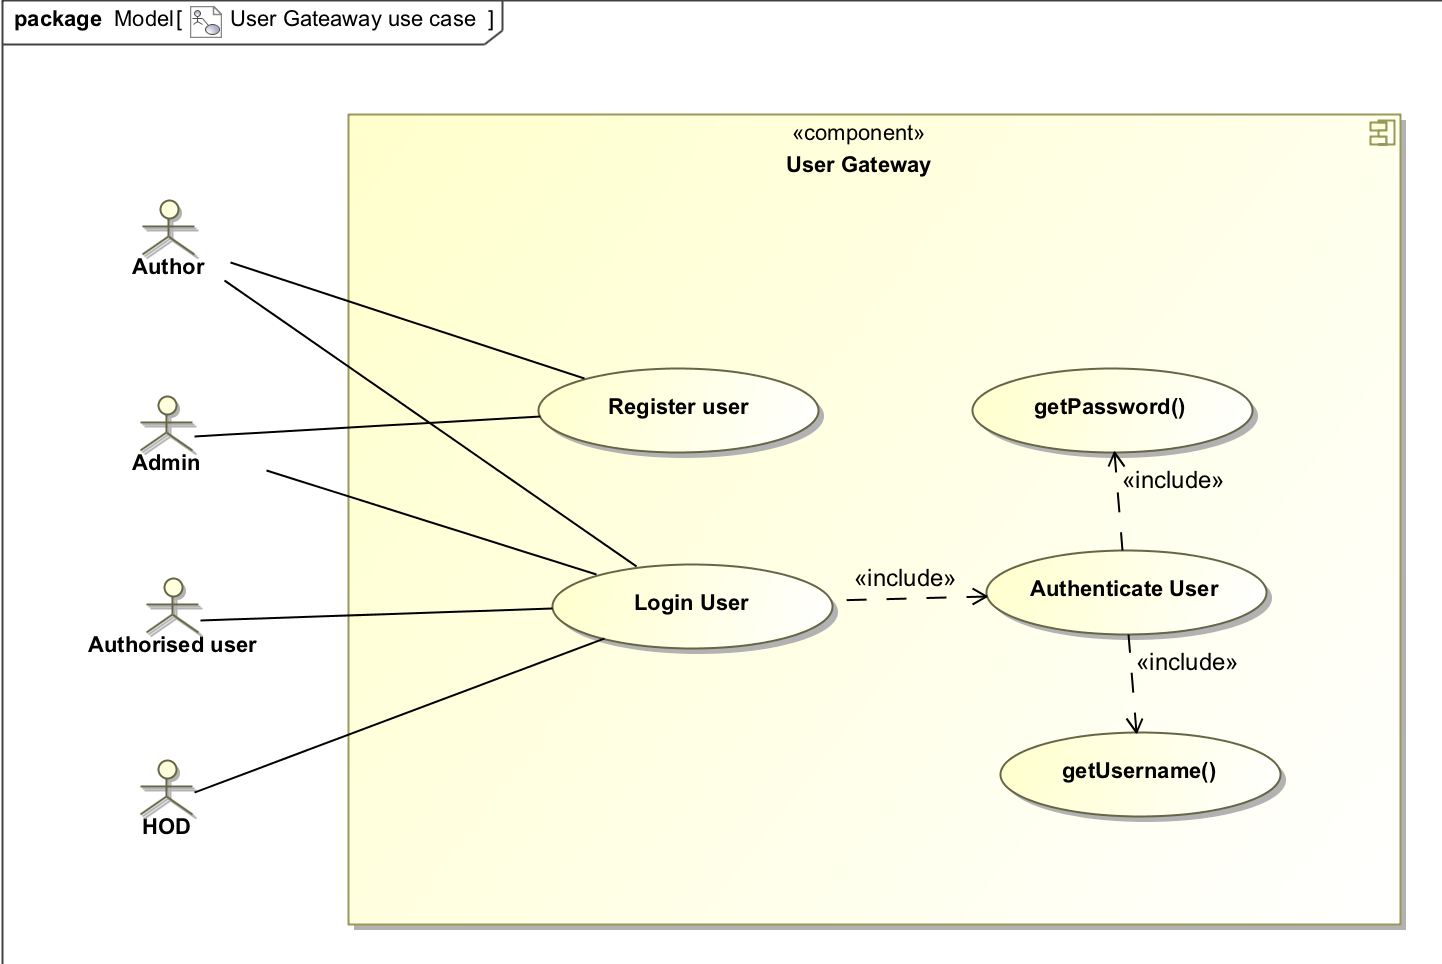
\includegraphics[width=\textwidth]{../Diagrams/UseCases/UserGateway_UseCase.png}\\[0.5cm]
	\end{center}
	\newpage
	\subsubsection{Research Paper Management}
	\begin{center}
		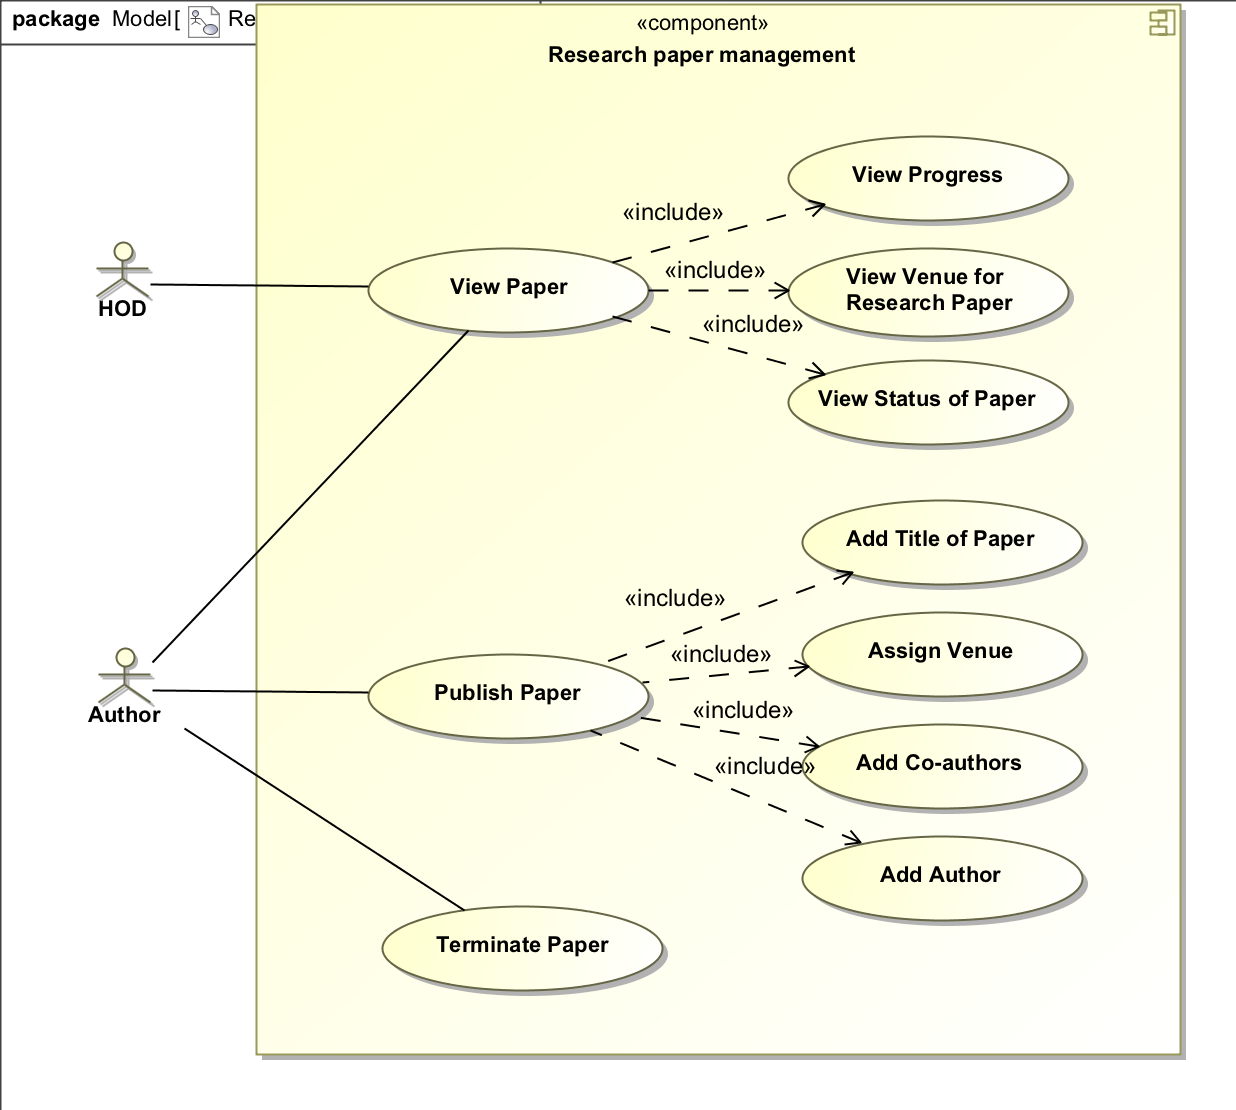
\includegraphics[width=\textwidth]{../Diagrams/UseCases/ResearchPaperManagement_UseCase.png}\\[0.5cm]
	\end{center}
	\newpage
	\subsubsection{User Account Management Services}
	\begin{center}
		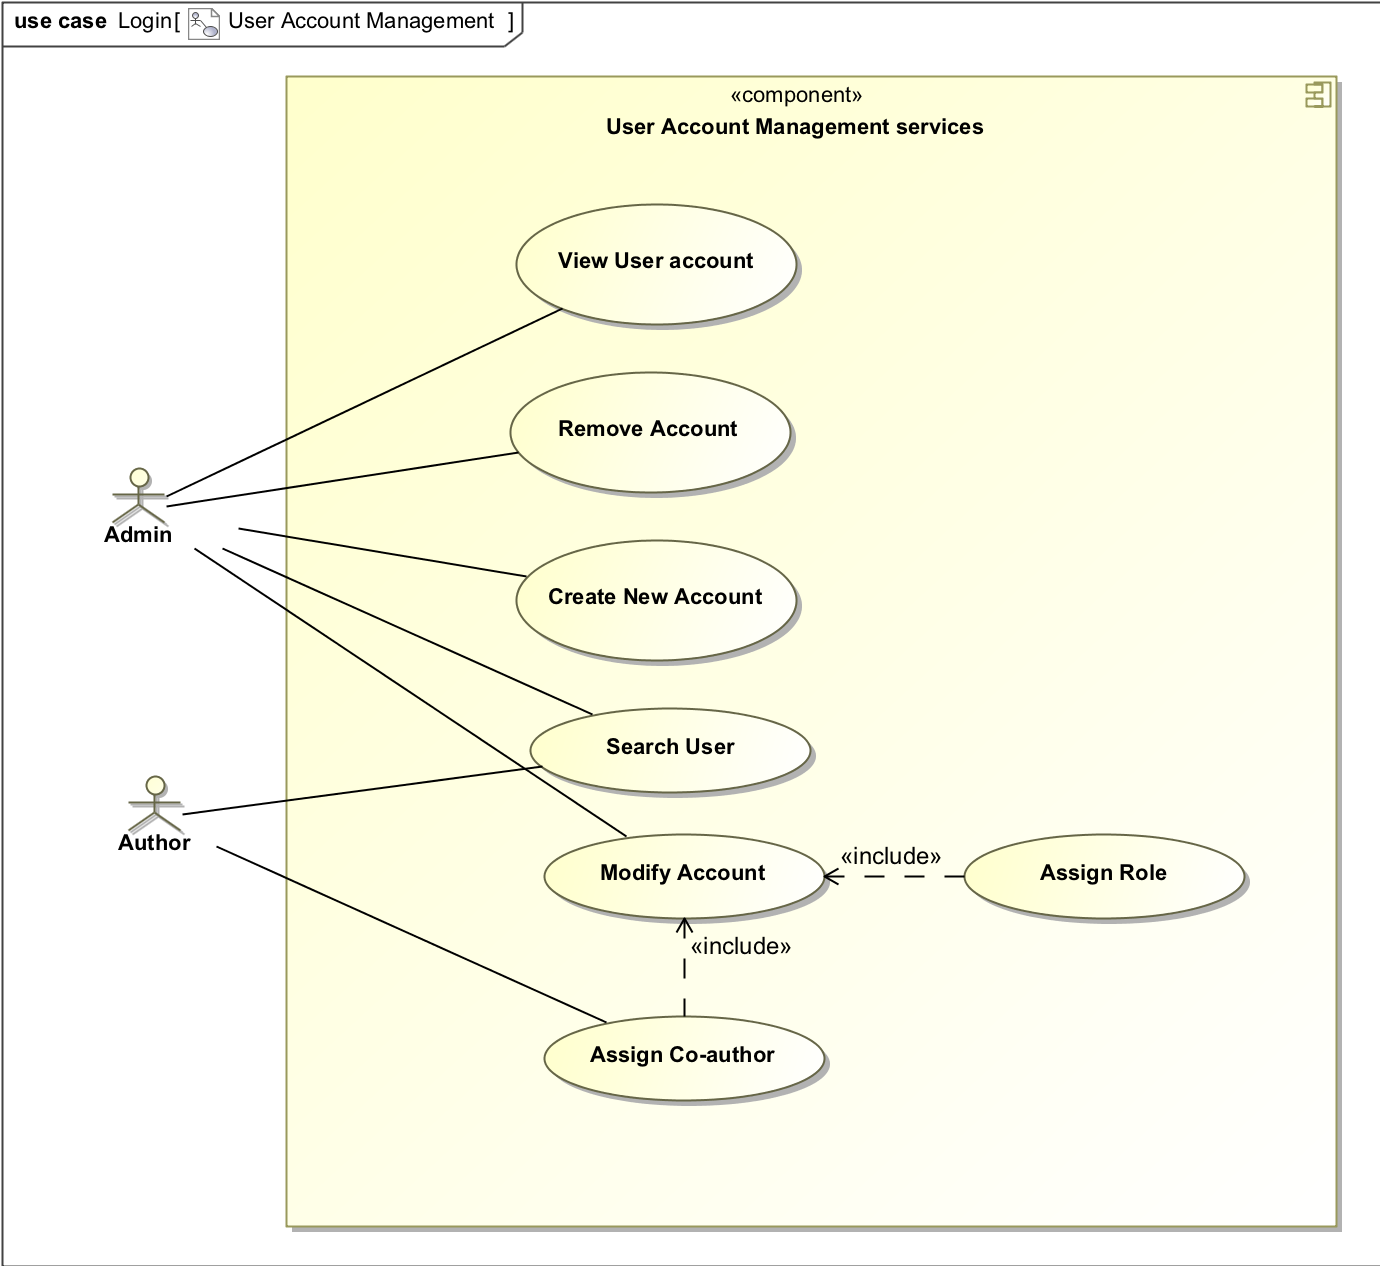
\includegraphics[width=\textwidth]{../Diagrams/UseCases/UserAccountManagementServices_UseCase.png}\\[0.5cm]
	\end{center}
	\newpage
	\subsubsection{Log Services}
	\begin{center}
		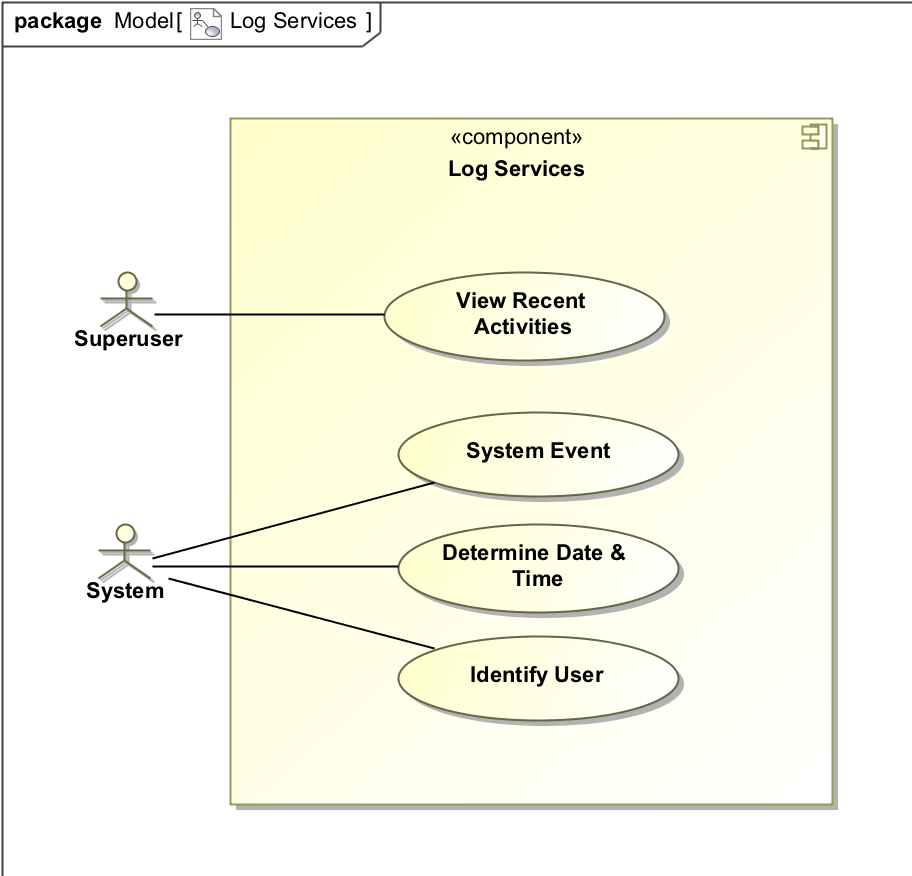
\includegraphics[width=\textwidth]{../Diagrams/UseCases/LogServices_UseCase.png}\\[0.5cm]
	\end{center}
	\newpage
	\subsubsection{Notification Services}
	\begin{center}
		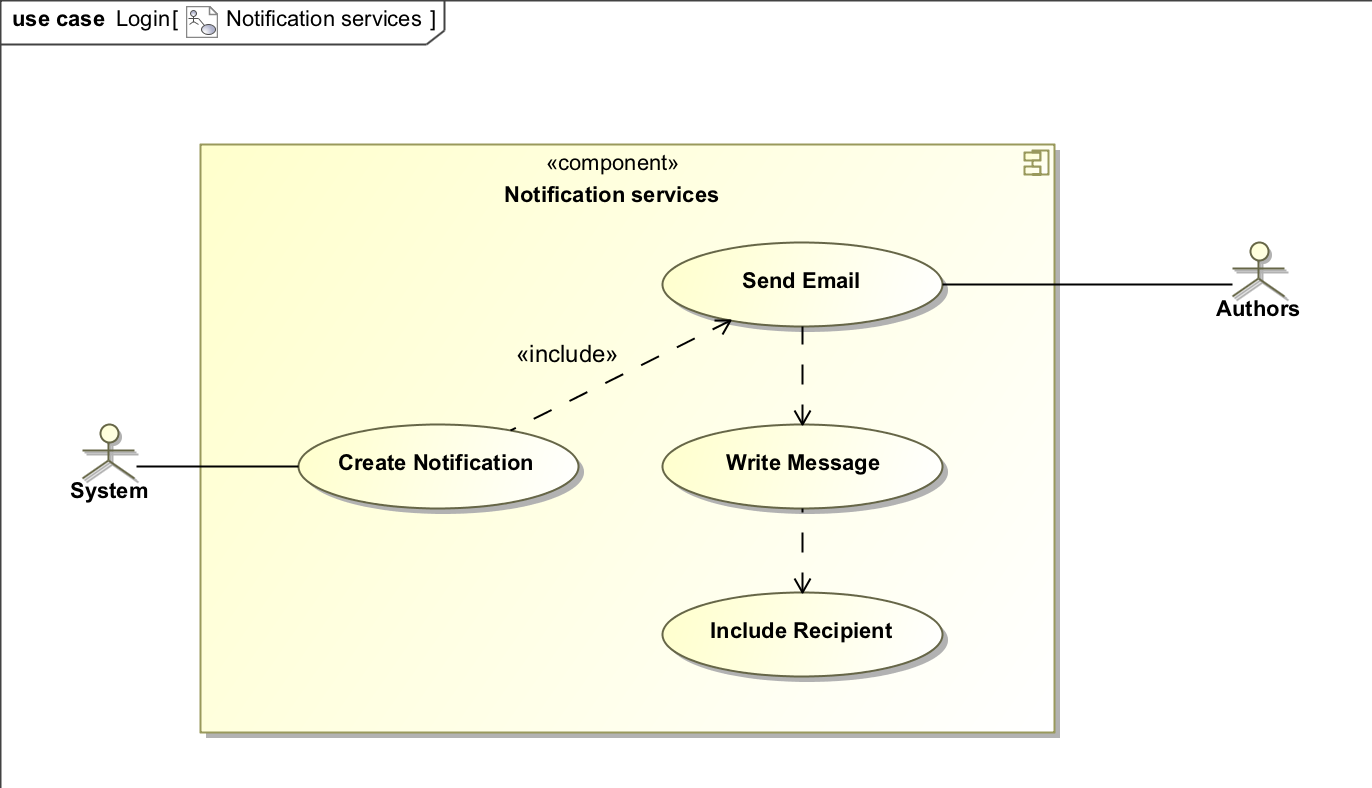
\includegraphics[width=\textwidth]{../Diagrams/UseCases/NotificationServices_UseCase.png}\\[0.5cm]
	\end{center}
	\newpage
	\subsubsection{Archival Services}
	\begin{center}
		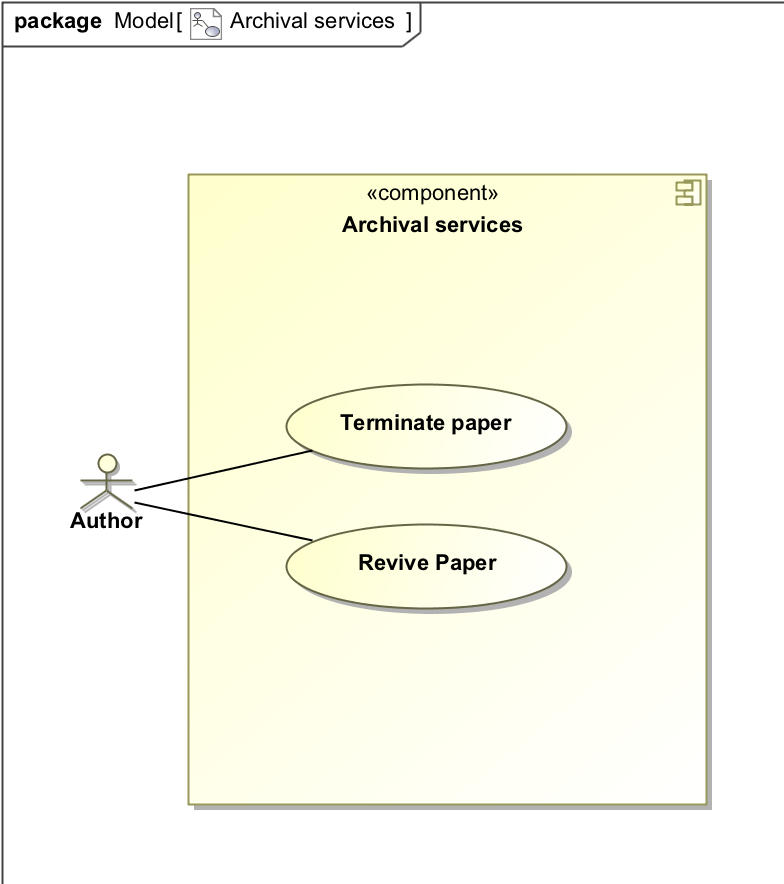
\includegraphics[width=\textwidth]{../Diagrams/UseCases/ArchivalServices_UseCase.png}\\[0.5cm]
	\end{center}
	\newpage
	
	\subsection{Process specifications}
	
	\subsubsection{Server Connection}
	\begin{center}
		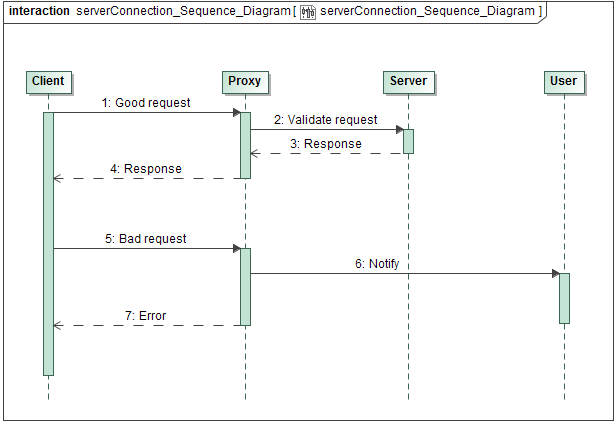
\includegraphics[width=\textwidth]{../Diagrams/SequenceDiagrams/Server_Connection_Sequence_Diagram.png}\\[0.5cm]
	\end{center}
	
	\newpage
	\subsubsection{Database Connection}
	\begin{center}
		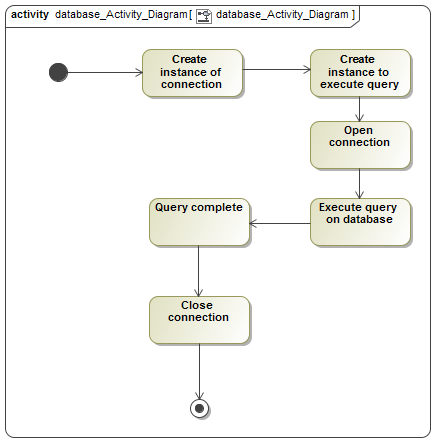
\includegraphics[width=\textwidth]{../Diagrams/ActivityDiagrams/database_Activity_Diagram.png}\\[0.5cm]
	\end{center}
	
	\newpage
	\subsubsection{Register User}
	\begin{center}
		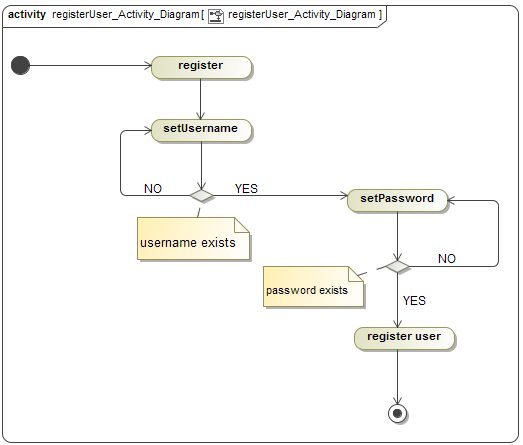
\includegraphics[width=\textwidth]{../Diagrams/ActivityDiagrams/registerUser_Activity_Diagram.png}\\[0.5cm]
	\end{center}

	\newpage
	\subsubsection{Login}
	\begin{center}
		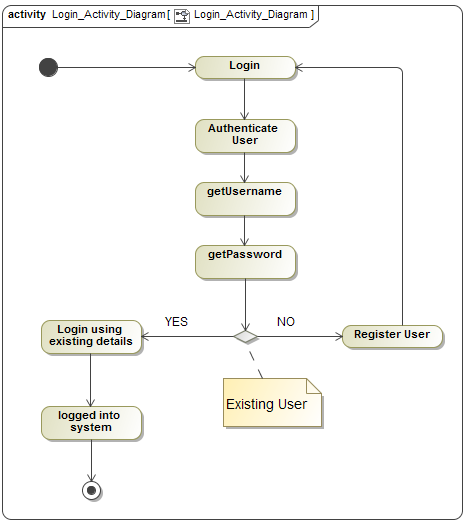
\includegraphics[width=\textwidth]{../Diagrams/ActivityDiagrams/Login_Activity_Diagram.png}\\[0.5cm]
	\end{center}
	

	\newpage
	\subsubsection{Add new User}
	\begin{center}
		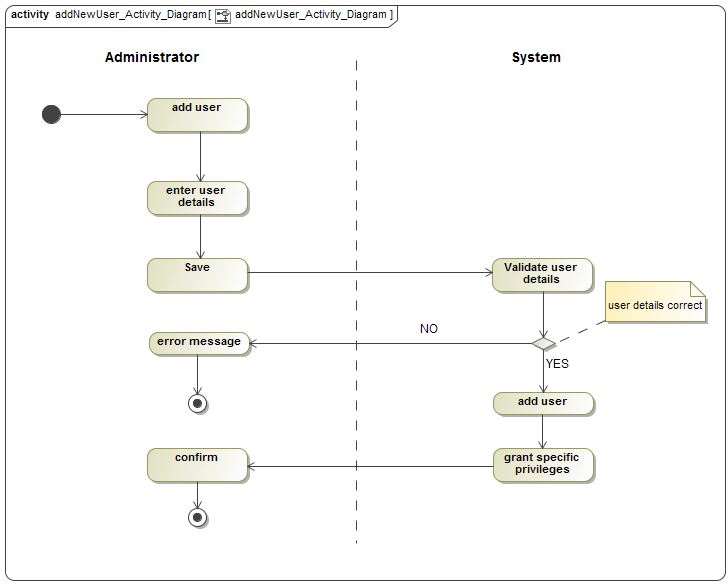
\includegraphics[width=\textwidth]{../Diagrams/ActivityDiagrams/addNewUser_Activity_Diagram.png}\\[0.5cm]
	\end{center}

	\newpage
	\subsubsection{View User Account}
	\begin{center}
		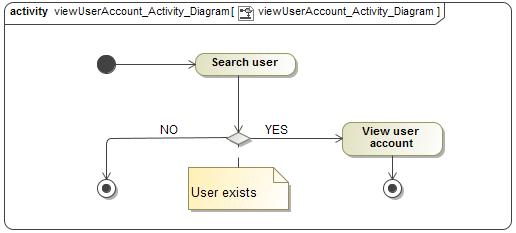
\includegraphics[width=\textwidth]{../Diagrams/ActivityDiagrams/viewUserAccount_Activity_Diagram.png}\\[0.5cm]
	\end{center}
	
	\newpage
	\subsubsection{Remove Account}
	\begin{center}
		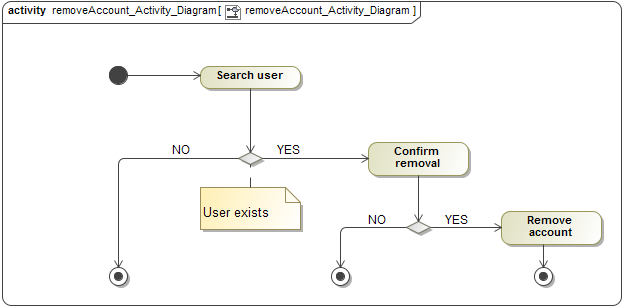
\includegraphics[width=\textwidth]{../Diagrams/ActivityDiagrams/removeAccount_Activity_Diagram.png}\\[0.5cm]
	\end{center}
	
	\newpage
	\subsection{Domain Model}
	\begin{center}
		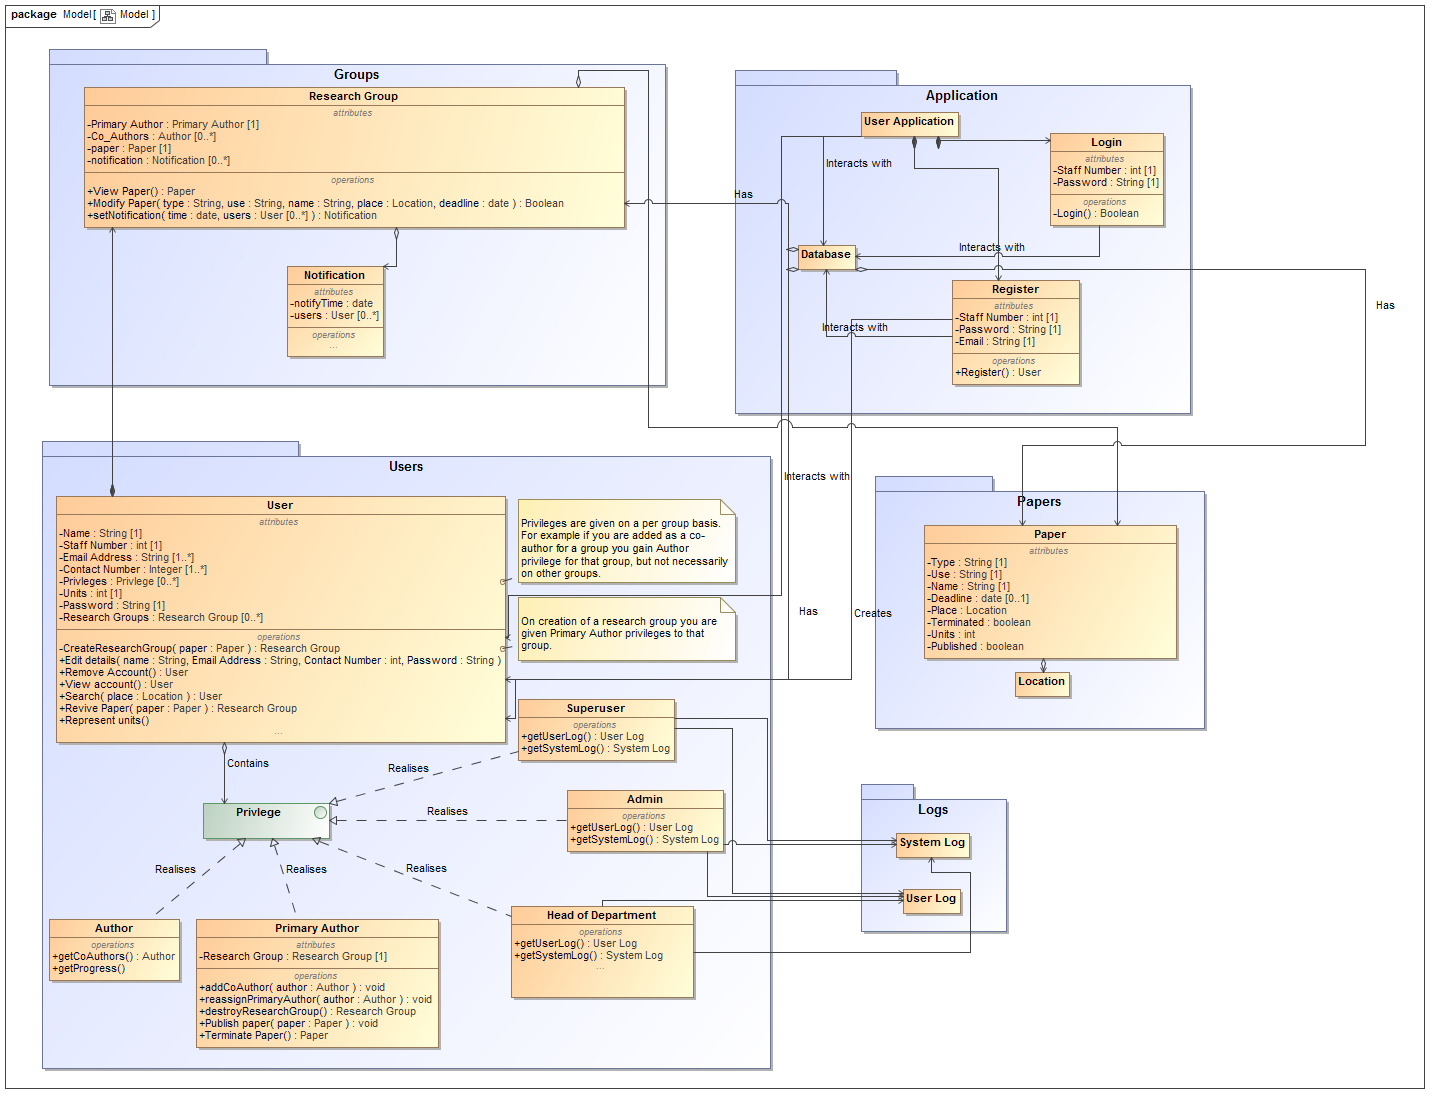
\includegraphics[width=\textwidth]{../Diagrams/DomainModel/Model.png}\\[0.5cm]
	\end{center}
	
	\newpage
	\section{Open Issues}
	\begin{itemize}
		\item For further references and to access Team Braovo's github repository, please click on this \href{https://github.com/ish1993/Bravo}{link}.
		\end{itemize}
		
	\newpage
	\addcontentsline{toc}{section}{References}
	\bibliographystyle{plainurl}
	\bibliography{bibfile}{}
	
\end{document}
